\documentclass[a4paper]{article}

\usepackage[english]{babel}
\usepackage[utf8x]{inputenc}
\usepackage{amsmath}
\usepackage{graphicx}
\usepackage[colorinlistoftodos]{todonotes}
\usepackage{hyperref}
\usepackage{listings}
\usepackage[numbers]{natbib}
\usepackage{babel,blindtext}
\usepackage{bbm}

\usepackage{algorithm}
\usepackage[noend]{algpseudocode}

\usepackage{booktabs} % To thicken table lines

\title{Learning to Trade Using Q-Learning}
\author{Uirá Caiado}

\begin{document}
\maketitle

\begin{abstract}
In this project, I will present an adaptive learning model to trade a single stock under the reinforcement learning framework. This area of machine learning consists in training an agent by reward and punishment without needing to specify the expected action. The agent learns from its experience and develops a strategy that maximizes its profits. The simulation results show initial success in bringing learning techniques to build algorithmic trading strategies.
\end{abstract}

%%%%%%%%%%%%%%%%%%%%%%%%%%%%%%%%%%%%%%%%%%%%%%%%%%%%%%%%%%%%%%%%%%%%%%%%%%%%%%%%%%%%%%%%
%% INTRODUCTION
%%%%%%%%%%%%%%%%%%%%%%%%%%%%%%%%%%%%%%%%%%%%%%%%%%%%%%%%%%%%%%%%%%%%%%%%%%%%%%%%%%%%%%%%

\section{Introduction}
\label{sec:introduction}

In this section, I will provide a high-level overview of the project, define the problem addressed and the metric used to measure the performance of the model created.

\subsection{Project Overview}
Nowadays, algo trading represents almost half of all cash equity trading in western Europe. In advanced markets, it already accounts\footnote{Source: \url{https://goo.gl/v2BENs}} for over 40\%-50\% of total volume. In Brazil its market share is not as large – currently about 10\% – but is expected to rise in the years ahead as markets and players go digital.

As automated strategies are becoming increasingly popular, building an intelligent system that can trade many times a day and adapts itself to the market conditions and still consistently makes money is a subject of keen interest of any market participant.

Given that it is hard to produce such strategy, in this project I will try to build an algorithm that just does better than a random agent, but learns by itself how to trade. To do so, I will feed my agent with four days of information about every trade and change in the top of the order book\footnote{Source: \url{https://goo.gl/k1dDYZ}} in the PETR4 - one of the most liquidity assets in Brazilian Stock Market - in a Reinforcement Learning Framework. Later on, I will test what it has learned in a newest dataset.

The dataset used in this project is also known as level I order book data\footnote{Source: \url{https://goo.gl/sP1viq}} and includes all trades and changes in the prices and total quantities at best Bid (those who wants to buy the stock) and Offer side (those who intends to sell the stock).


\subsection{Problem Statement}
Algo trading\footnote{Source: \url{http://goo.gl/b9jAqE}} strategies usually are programs that follow a predefined set of instructions to place its orders. The primary challenge to this approach is building these rules in a way that it can consistently generate profit without being too sensitive to market conditions.

Thus, the goal of this project is to develop an adaptive learning model that can learn by itself those rules and trade a particular asset using reinforcement learning framework under an environment that replays historical high-frequency data.

As \cite{chan2001electronic} described, reinforcement learning can be considered as a model-free approximation of dynamic programming. The knowledge of the underlying processes is not assumed but learned from experience.

The agent can access some information about the environment state as the order flow imbalance, the sizes of the best bid and offer and so on. At each time step $t$, It should generate some valid action, as buy stocks or insert a limit order at the Ask side. All inputs and actions will be detailed in the next sections.

The agent also should receive a reward or a penalty at each time step if it is already carrying a position from previous rounds or if it has made a trade (the cost of the operations are computed as a penalty).

Based on the rewards and penalties it gets, the agent should learn an optimal policy for trade this particular stock, maximizing the profit it receives from its actions and resulting positions.

\subsection{Metrics}
In 1988, the Wall Street Journal created a Dartboard Contest\footnote{Source: \url{http://www.automaticfinances.com/monkey-stock-picking/}}, where Journal staffers threw darts at a stock table to select their assets, while investment experts picked their own stocks. After six months, they compared the results of the two methods. After adjusting the results to risk level, they found out that the pros barely have beaten the random pickers.

Given that, the metric used to measure the performance of the learner will be the amount of money made by a random agent. So, my goal will be to outperform this agent, that should just produce some random action from a set of allowed action at each time $t$. In the next section, I will detail the behavior of this agent.

%%%%%%%%%%%%%%%%%%%%%%%%%%%%%%%%%%%%%%%%%%%%%%%%%%%%%%%%%%%%%%%%%%%%%%%%%%%%%%%%%%%%%%%%
%% ANALYSIS
%%%%%%%%%%%%%%%%%%%%%%%%%%%%%%%%%%%%%%%%%%%%%%%%%%%%%%%%%%%%%%%%%%%%%%%%%%%%%%%%%%%%%%%%

\section{Analysis}
\label{sec:analysis}

In this section, I will explore the data set that will be used in the simulation, define and justify the inputs employed in the state representation of the algorithm, explain the reinforcement learning techniques used and provide a benchmark.

\subsection{Data Exploration}
The dataset used is composed by level I order book data from PETR4, a stock traded at BMFBovespa Stock Exchange. Includes 19 trading sessions from 07/25/2016 to 09/26/2016. I will use one day to create the scalers of the features used, that I shall explain. Then, I will use four days to train and test the model, and after each training session, I will validate the policy found in an unseen dataset from the subsequent day. The data was collected from Bloomberg. There are 45 files, each one has 110,000 rows on average, resulting in 5,631,273 rows at total and almost  230 MB of information. In the figure \ref{tab:original_data} is the structure of one of them:

\begin{table}[ht!]
\centering
\begin{tabular}{l|llrr}
{} &                Date &   Type &  Price &   Size \\
\midrule
0 & 2016-07-25 10:02:00 &  TRADE &  11.98 &   5800 \\
1 & 2016-07-25 10:02:00 &    BID &  11.97 &   6100 \\
2 & 2016-07-25 10:02:00 &    ASK &  11.98 &  51800 \\
3 & 2016-07-25 10:02:00 &    ASK &  11.98 &  56800 \\
4 & 2016-07-25 10:02:00 &    ASK &  11.98 &  56900 \\

\end{tabular}
\caption{\label{tab:original_data}Basic Structure of the Files}
\end{table}

Each file is composed of four different fields. The column $Date$ is the time-stamp of the row and has a precision of seconds. $Type$ is the kind of information that the row encompasses. The type 'TRADE' relates to an actual trade that has happened. 'BID' is related to changes in the best Bid level and 'ASK', to the best Offer level. $Price$ is the current best bid or ask and $Size$ is the accumulated quantity on that price and side.

All this data will be used to create the environment where my agent will operate. This environment is an order book, where the agent will be able to insert limit orders and execute trades at the best prices. The order book (figure \ref{tab:order_book}) is represented by two binary trees, one for the Bid and other for the Ask side. As can be seen in the table below, the nodes of these trees are sorted by price (price level) in ascending order on the Bid side and descending order on the ask side. At each price level, there are other binary trees sorted by order of arrival. The first order to arrive is the first order filled when coming in a trade.

\begin{table}[ht!]
\centering
\begin{tabular}{l|lrrl}
{} &    qBid &    Bid &    Ask &    qAsk \\
\midrule
0 &  61,400 &  12.02 &  12.03 &  13,800 \\
1 &  47,100 &  12.01 &  12.04 &  78,700 \\
2 &  51,700 &  12.00 &  12.05 &  20,400 \\
3 &  37,900 &  11.99 &  12.06 &  23,100 \\
4 &  97,000 &  11.98 &  12.07 &  27,900 \\

\end{tabular}
\caption{\label{tab:order_book}Order Book Example}
\end{table}

The environment will answer with the agent's current position and Profit and Loss (PnL) every time the agent executes a trade or has an order filled. The cost of the trade will be accounted as a penalty.

The agent also will be able to sense the state of the environment and include it in its own state representation. So, this intern state will be represented by a set of variables about the current situation of the market and the state of the agent, given by:

\begin{itemize}
\item $qOFI$ : integer. The net order flow in the last 10 seconds
\item $book\_ratio$ : float. The Bid size over the Ask size
\item $position$: integer. The current position of my agent
\item $OrderBid$: boolean. If the agent has order at the bid side
\item $OrderAsk$: boolean. If the agent has order at the ask side
\end{itemize}

Regarding the measure of the Order Flow Imbalance (OFI), there are many ways to measure it. \cite{cont2014price} argued the *order flow imbalance* is a measure of supply/demand imbalance and defines it as a sum of individual event contribution $e_n$ over time intervals $\left[ t_{k-1}, \; t_k \right]$, such that:
$$OFI_k = \sum^{N(t_k)}_{n=N(t_{k-1})+1} e_n$$

Where $N(t_k)$ and $N(t_{k-1}) + 1$ are index of the first and last event in the interval. The $e_n$ was defined by the authors as a measure of the contribution of the $n$-th event to the size of the bid and ask queues:
$$e_n = \mathbbm{1}_{P_{n}^{B} \geq P_{n-1}^{B}} q^{B}_{n} - \mathbbm{1}_{P_{n}^{B} \leq P_{n-1}^{B}}  q^{B}_{n-1} - \mathbbm{1}_{P_{n}^{A} \leq P_{n-1}^{A}} q^{A}_{n} + \mathbbm{1}_{P_{n}^{A} \geq P_{n-1}^{A}}  q^{A}_{n-1}$$

Where $q^{B}_{n}$ and $q^{A}_{n}$ are linked to the accumulated quantities at the best bid and ask in the time $n$. The subscript $n-1$ is related to the last observation. $\mathbbm{1}$ is an indicator\footnote{Source: \url{https://en.wikipedia.org/wiki/Indicator_function}} function. In the figure below is plotted the 10-second log-return of PETR4 against the contemporaneous OFI.

\begin{figure}[ht!]
\centering
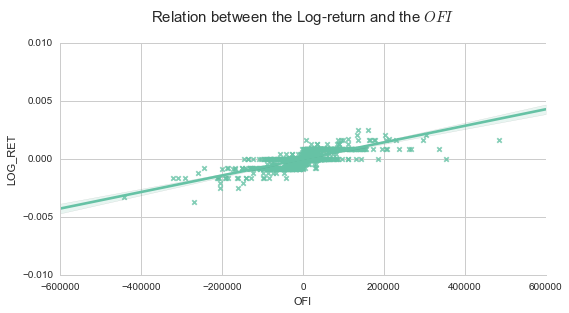
\includegraphics[width=0.75\textwidth]{figures/ofi_logret.png}
\caption{\label{fig:ofi_linear}10-second log-return against OFI}
\end{figure}

As described by \cite{cont2014price} in a similar test, the figure \ref{fig:ofi_linear} suggests that order flow imbalance is a stronger driver of high-frequency price changes and this variable will be used to describe the current state of the order book.

\subsection{Algorithms and Techniques}
Based on \cite{cont2014price}, the algo trading might be conveniently modeled in the framework of reinforcement learning. As suggested by \cite{du1algorithm}, this framework adjusts the parameters of an agent to maximize the expected payoff or reward generated due to its actions. Therefore, the agent learns a policy that tells him the actions it must perform to achieve its best performance. This optimal policy is exactly what we hope to find when we are building an automated trading strategy.

According to \cite{chan2001electronic}, Markov decision processes (MDPs) are the most common model when implementing reinforcement learning.  The MDP model of the environment consists, among other things, of a discrete set of states $S$ and a discrete set of actions taken from $A$. In this project, depending on the position of the learner(long or short), at each time step $t$ it will be allowed to choose an action $a_t$ from different subsets from the action space $A$ , that consists of six possibles actions:
$$a_t \in \left (None,\, buy,\, sell,\, best\_bid,\, best\_ask,\, best\_both \right)$$

Where $None$ indicates that the agent shouldn't have any order in the market. $Buy$ and $Sell$ means that the agent should execute a market order to buy or sell $100$ stocks (the size of an order will always be a hundred shares). This kind of action will be allowed based on a trailing stop\footnote{Source: \url{https://goo.gl/SVmVzJ}} of 4 cents. $best\_bid$ and $best\_ask$ indicate that the agent should keep order at best price just in the mentioned side and $best\_both$, it should have ordered at best price in both sides.

So, at each discrete time step $t$, the agent senses the current state $s_t$ and choose to take an action $a_t$. The environment responds by providing the agent a reward $r_t=r(s_t, a_t)$ and by producing the succeeding state $s_{t+1}=\delta(s_t, a_t)$. The functions $r$ and $\delta$ only depend on the current state and action (it is memoryless\footnote{Source: \url{https://en.wikipedia.org/wiki/Markov_process}}, are part of the environment and are not necessarily known to the agent.

The task of the agent is to learn a policy $\pi$ that maps each state to an action ($\pi: S \rightarrow A$), selecting its next action $a_t$ based solely on the current observed state $s_t$, that is $\pi(s_t)=a_t$. The optimal policy, or control strategy, is the one that produces the greatest possible cumulative reward over time. So, stating that:
$$V^{\pi}(s_t)= r_t + \gamma r_{t+1} + \gamma^2 r_{t+1} + ... = \sum_{i=0}^{\infty} \gamma^{i} r_{t+i}$$

Where $V^{\pi}(s_t)$ is also called the discounted cumulative reward and it represents the cumulative value achieved by following an policy $\pi$ from an initial state $s_t$ and $\gamma \in [0, 1]$ is a constant that determines the relative value of delayed versus immediate rewards. It is one of the

If we set $\gamma=0$, only immediate rewards is considered. As $\gamma \rightarrow 1$, future rewards are given greater emphasis relative to immediate reward. The optimal policy $\pi^{*}$ that will maximizes $V^{\pi}(s_t)$ for all states $s$ can be written as:
$$\pi^{*} = \underset{\pi}{\arg \max} \, V^{\pi} (s)\,\,\,\,\,, \,\, \forall s$$

However, learning $\pi^{*}: S \rightarrow A$ directly is difficult because the available training data does not provide training examples of the form $(s, a)$. Instead, as \cite{Mitchell} explained, the only available information is the sequence of immediate rewards $r(s_i, a_i)$ for $i=1,\, 2,\, 3,\,...$

So, as we are trying to maximize the cumulative rewards $V^{*}(s_t)$ for all states $s$, the agent should prefer $s_1$ over $s_2$ wherever $V^{*}(s_1) > V^{*}(s_2)$. Given that the agent must choose among actions and not states, and it isn't able to perfectly predict the immediate reward and immediate successor for every possible state-action transition, we also must learn $V^{*}$ indirectly.

To solve that, we define a function $Q(s, \, a)$ such that its value is the maximum discounted cumulative reward that can be achieved starting from state $s$ and applying action $a$ as the first action. So, we can write:
$$Q(s, \, a) = r(s, a) + \gamma V^{*}(\delta(s, a))$$

As $\delta(s, a)$ is the state resulting from applying action $a$ to state $s$ (the successor) chosen by following the optimal policy, $V^{*}$ is the cumulative value of the immediate successor state discounted by a factor $\gamma$. Thus,  what we are trying to achieve is
$$\pi^{*}(s) = \underset{a}{\arg \max} Q(s, \, a)$$

It implies that the optimal policy can be obtained even if the agent just uses the current action $a$ and state $s$ and chooses the action that maximizes $Q(s,\, a)$. Also, it is important to notice that the function above implies that the agent can select optimal actions even when it has no knowledge of the functions $r$ and $\delta$.

Lastly, according to \cite{Mitchell}, there are some conditions to ensure that the reinforcement learning converges toward an optimal policy. On a deterministic MDP, the agent must select actions in a way that it visits every possible state-action pair infinitely often. This requirement can be a problem in the environment that the agent will operate.

As the most inputs suggested in the last subsection was defined in an infinite space, in section \ref{sec:methodology} I will discretize those numbers before use them to train my agent, keeping the state space representation manageable, hopefully. We also will see how \cite{Mitchell} defined a reliable way to estimate training values for $Q$, given only a sequence of immediate rewards $r$.

\subsection{Benchmark}
As described before, the performance of my agent will be compared to the performance of a random agent. This random agent should select a random action from a set of valid actions taken from $A$ at each time step $t$.

Just like my learner, the set of action can change over time depending on the open position, that is limited to $100$ stocks at most, on any side. When it reaches its limit, it will be allowed just to perform actions that decrease its position. So, for instance, if it already long\footnote{Source: \url{https://goo.gl/GgXJgR}} in $100$ shares, the possible moves would be $\left (None,\, sell,\, best\_ask \right)$. If it is short\footnote{Source: \url{https://goo.gl/XFR7q3}}, it just can perform $\left (None,\, buy,\, best\_bid\right)$.

The performance will be measured primarily in the money made by the agents (that will be optimized by the learner). First, I will analyze if the learning agent was able to improve its performance on the same dataset after different trials. Later on, I will use the policy learned to simulate the learning agent behavior in a different dataset and then I will compare the final Profit and Loss and volatility of the returns of both agents. All data analyzed will be obtained by simulation.

%%%%%%%%%%%%%%%%%%%%%%%%%%%%%%%%%%%%%%%%%%%%%%%%%%%%%%%%%%%%%%%%%%%%%%%%%%%%%%%%%%%%%%%%
%% METHODOLOGY
%%%%%%%%%%%%%%%%%%%%%%%%%%%%%%%%%%%%%%%%%%%%%%%%%%%%%%%%%%%%%%%%%%%%%%%%%%%%%%%%%%%%%%%%

\section{Methodology}
\label{sec:methodology}

In this section, I will discretize the input space and implement an agent to learn the Q function.

\subsection{Data Preprocessing}
As mentioned before, I will implement a Markov decision processes (MDP) that requires, among other things, of a discrete set of states $S$. Apart from the input variables $position$, $OrderBid$, $OrderAsk$, the other variables are defined in an infinite domain. I am going to discretize those inputs, so my learning agent can use them in the representation of their intern state. In the Figure \ref{fig:features_one}, we can see the distribution of those variables. The data was produced using the first day of the dataset.


\begin{figure}[ht!]
\minipage{0.49\textwidth}
  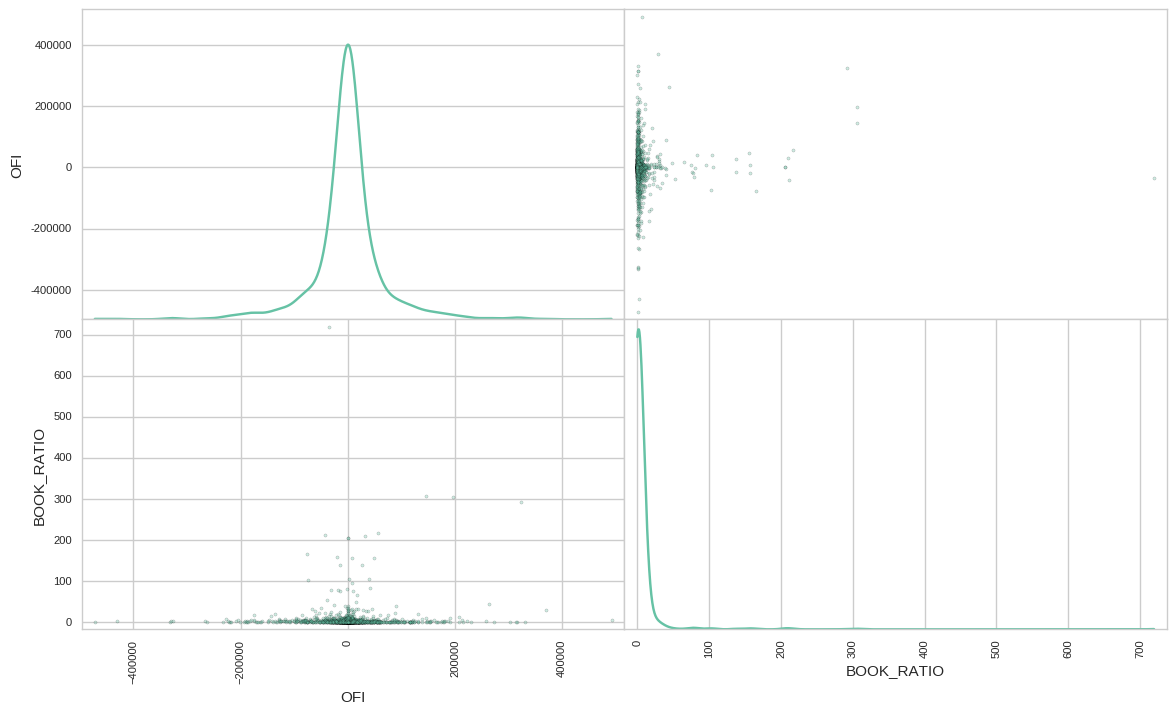
\includegraphics[width=\linewidth]{figures/scatter_feat_1.png}
  \caption{\label{fig:features_one}Exploration vs Exploitation}
\endminipage
\minipage{0.49\textwidth}
  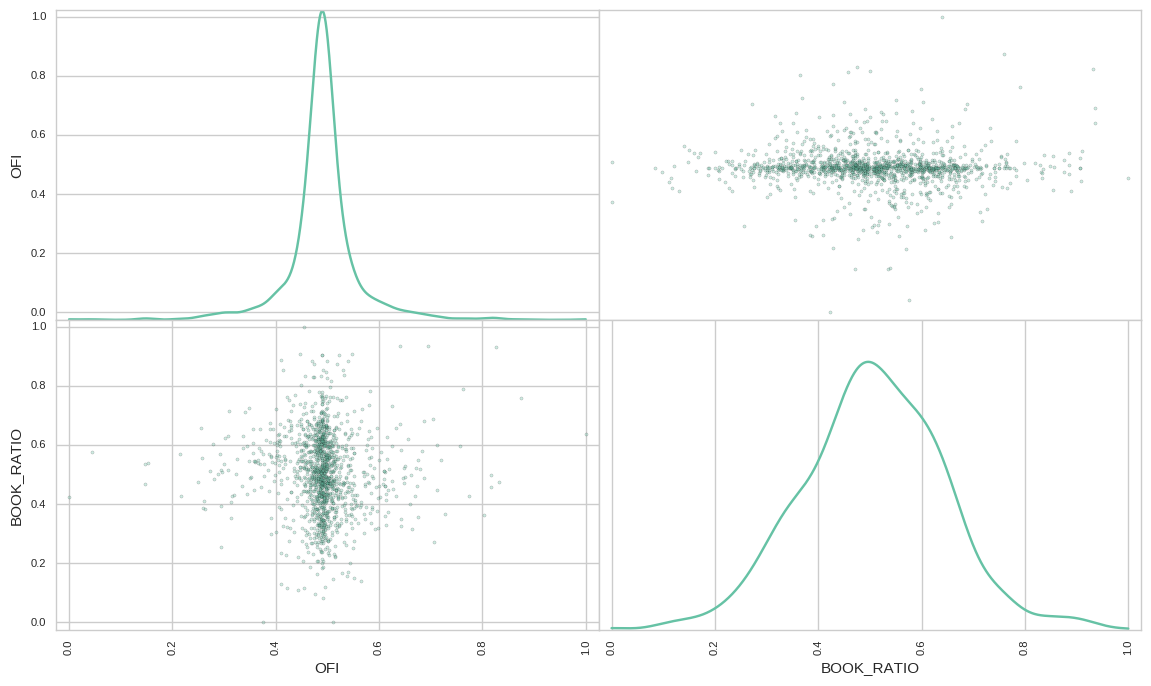
\includegraphics[width=\linewidth]{figures/scatter_feat_2.png}
  \caption{\label{fig:features_two}On Time Ratio}
\endminipage
\end{figure}

The scale of the variables is very different, and, in the case of the Book Ratio, it presents a logarithmic distribution. I will apply a logarithm transformation on this variable and re-scale both to lie between a given minimum and maximum value of each feature using the function MinMaxScaler\footnote{Source: \url{http://scikit-learn.org/stable/modules/preprocessing.html}} from scikit-learn. The result of the transformation can be seen in the figure \ref{fig:features_two}.

As mentioned before, in an MDP environment the agent must visit every possible state-action pair infinitely often. If I just bucketize the variables and combine them, I will end up with a huge number of states to explore. So, to reduce the state space, I am going to group those variables using K-Means and Gaussian Mixture Model (GMM) clustering algorithm. Then I will quantify the "goodness" of the clustering results by calculating each data point's silhouette coefficient\footnote{Source: \url{https://goo.gl/FUVD50}}. The silhouette coefficient for a data point measures how similar it is to its assigned cluster from -1 (dissimilar) to 1 (similar). In the figure \ref{fig:scores}, I am going to calculate the mean silhouette coefficient to K-Means and GMM using a different number of clusters. Also, I will test different covariance structures to GMM.

\begin{figure}[ht]
\centering
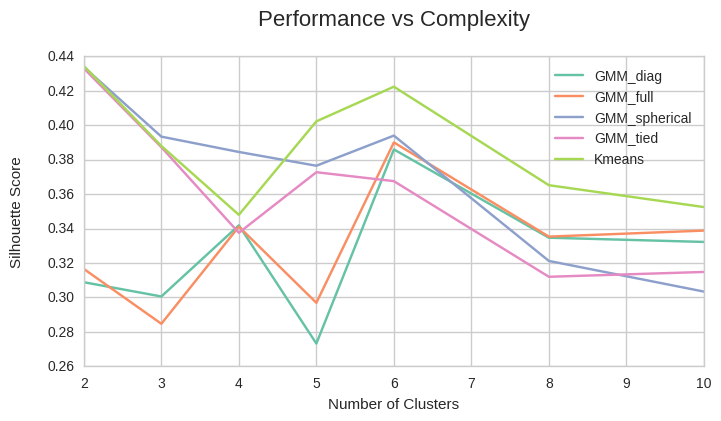
\includegraphics[width=0.65\textwidth]{figures/cluster_scores.png}
\caption{\label{fig:scores}Silhouette Scores.}
\end{figure}

The maximum score has happened using two clusters. However, I believe that the market can't be simplified that much. So, I will use the K-means with six centroids to group the variables. In the figure \ref{fig:clusters} we can see how the algorithm classified the data. Also, in the table \ref{tab:cluster_recover}, the centroid was put in their original scales.

\begin{figure}[ht]
\centering
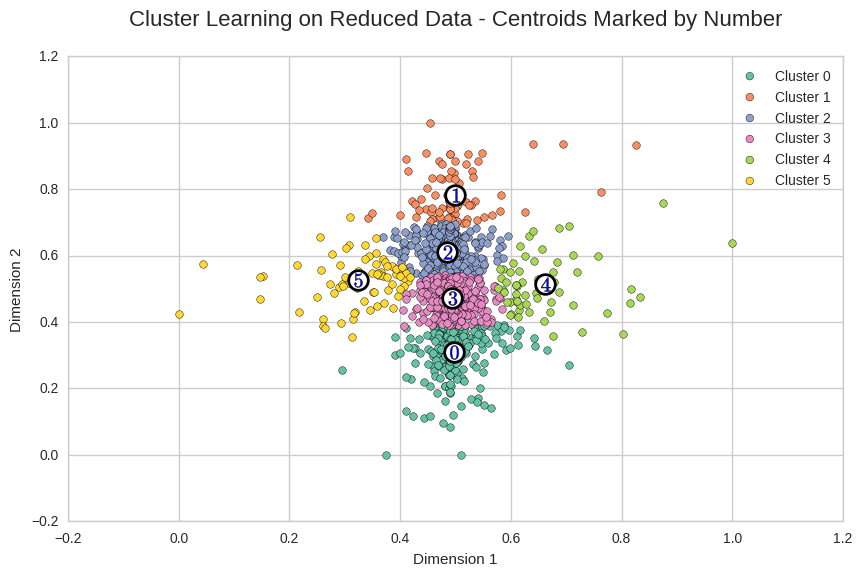
\includegraphics[width=0.65\textwidth]{figures/cluster_scatter.png}
\caption{\label{fig:clusters}Clusters Found.}
\end{figure}

\begin{table}[ht!]
\centering
\begin{tabular}{l|rr}
{Cluster} &    BOOK\_RATIO &    OFI \\
\midrule
0 &  0.89 &  -173,662 \\
1 &  0.91 &  281,563 \\
2 &  0.76 &  116,727 \\
3 &  0.85 &  -16,602 \\
4 &  7.91 &  23,334 \\
5 &  0.09 &  34,240 \\

\end{tabular}
\caption{\label{tab:cluster_recover}Recovering Data From Centroids}
\end{table}

Curiously, the algorithm gave more emphasis on the $BOOK\_RATIO$  when its value was very large (the bid size almost eight times greater than the ask size) or tiny (when the bid size was one tenth of the ask size). The other cluster seems mostly dominated by the $OFI$. In the next subsection, I will discuss how I have implemented the Q-learning, how I intend to perform the simulations and make some tests.


\subsection{Implementation}
As we have seen, learning the Q function corresponds to learning the optimal policy. According to \cite{Mohri_2012}, the optimal state-action value function $Q^{*}$ is defined for all $(s, \, a) \in S \times A$ as the expected return for taking the action $a \in A$ at the state $s \in S$, following the optimal policy. So, it can be written as \cite{Mitchell} suggested:

$$V^{*}(s) = \underset{a'}{\arg \max} \, Q(s, \, a')$$

Using this relationship, we can write a recursive definition of Q function, such that:

$$Q(s, \, a) = r(s, a) + \gamma \, \underset{a'}{\max} \, Q(\delta(s,\, a), \, a')$$

The recursive nature of the function above implies that our agent doesn't know the actual $Q$ function. It just can estimate $Q$, that we will refer as $\hat{Q}$. It will represents is hypothesis $\hat{Q}$ as a large table that attributes each pair $(s\, , \, a)$ to a value for $\hat{Q}(s,\, a)$ - the current hypothesis about the actual but unknown value $Q(s, \, a)$. I will initialize this table with zeros, but it could be filled with random numbers, according to \cite{Mitchell}. Still according to him, the agent repeatedly should observe its current state $s$ and do the following:

\begin{algorithm}
\caption{Update Q-table}\label{alg:qtable}
\begin{algorithmic}[1]
\Loop{ Observe the current state $s$ and the allowed actions $A^{*}$ and:}
  \State Choose some action $a$ and execute it
  \State Receive the immediate reward $r = r(s, a)$
  \State initialize the table entry $\hat{Q}(s, \, a)$ to zero if there is no entry $(s, \, a)$
  \State Observe the new state $s' = \delta(s, \,a)$
  \State Updates the table entry for $\hat{Q}(s, \, a)$ following:

    \do $\hat{Q}(s, \, a) \leftarrow r + \gamma \, \underset{a'}{\max}\, \hat{Q}(s', \, a')$
  \State $s \leftarrow s'$
\EndLoop
\end{algorithmic}
\end{algorithm}

in the simulation, failing to explore other actions that could present even higher values. \cite{Mitchell} proposed to use a probabilistic approach to select actions, assigning higher probabilities to action with high $\hat{Q}$ values, but given to every action at least a nonzero probability. So, I will implement the following relation:

$$P(a_i\, | \,s ) = \frac{k ^{\hat{Q}(s, a_i)}}{\sum_j k^{\hat{Q}(s, a_j)}}$$

Where $P(a_i\, | \,s )$ is the probability of selecting the action $a_i$ given the state $s$. The constant $k$ is positive and determines how strongly the selection favors action with high $\hat{Q}$ values. Let's look at the number of times the algorithm choose to explore when we vary the value of the $k$.

Ideally, to optimize the policy found, the agent should iterate over the same dataset repeatedly until it is not able to improve its PnL. Later on, the policy learned will be tested against the same dataset to check its consistency. Lastly, this policy will be tested on the subsequent day of the training session. So, before perform the out-of-sample test, we will use the following procedure:

\begin{algorithm}
\caption{Train-Test Q-Learning Trader}\label{alg:qtrader}
\begin{algorithmic}[1]
\Loop{ each trial in total iterations desired:}
  \Loop{ each observation in the session:}
    \State Update the table $\hat{Q}$
  \EndLoop
  \State Save the table $\hat{Q}$ indexed by the trial ID
\EndLoop
\Loop{ each trial in total iterations desired:}
  \State Load the table $\hat{Q}$ related to the current trial
  \Loop{ each observation in the session:}
    \Loop{ Observe the current state $s$ and the allowed actions $A^{*}$ and:}
	  \If{$s \, \notin  \, \hat{Q}$}
      	\State Close out open positions or do nothing
      \Else
        \State Choose the optimal action $a \, \in \, A^{*}$ and execute it
      \EndIf
    \EndLoop
  \EndLoop
\EndLoop
\end{algorithmic}
\end{algorithm}

Each training session will include data from the largest part of a trading session, starting at 10:30 and closing at 16:30. Also, the agent will be allowed to hold a position of just 100 shares at maximum (long or short). When the training session is over, all positions from the learner will be closed out so the agent always will start a new session without carrying positions.

The agent will be allowed to take action every 2 seconds and, due to this delay, every time it decides to insert limit orders, it will place it 1 cent worst than the best price. So, if the best bid is $12.00$ and the best ask is $12.02$, if the agent chooses the action $BEST\_BOTH$, it should include a buy order at $11.99$ and a sell order at $12.03$. It will be allowed to cancel these orders after 2 seconds. However, if these orders are filled in the mean time, the environment will inform the agent so it can update its current position. Even though, it just will take new actions after passed those 2 seconds.

In the next subsection, I will try different configurations of $k$ and $\gamma$ to try to improve the performance of the learning agent over the same trial.

\subsection{Refinement}
As mentioned before, we should iterate over the same dataset and check the policy learned on the same observations until convergence. Given the time required to perform each train-test iteration, "until convergence" will be 10 repetitions. We are going to train the model on the dataset from 08/15/2016. After each iteration, we will check how the agent would perform using the policy it has just learned. The agent in the first training session will use $\gamma=0.7$ and $k=0.3$. In the figure below are the results of the first round of iterations:

\begin{figure}[ht]
\centering
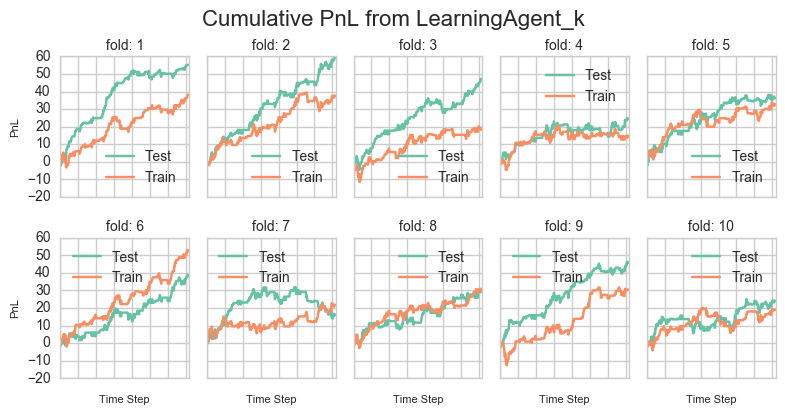
\includegraphics[width=0.75\textwidth]{figures/policy_tests_1.png}
\caption{\label{fig:policy_test_1}The PnL Curves Using each Policy Learned.}
\end{figure}

The curve Train in the charts is the PnL obtained during the training session when the agent was allowed to explore new actions randomly. The test is the PnL obtained using strictly the policy learned.

Although the agent was able to profit at the end of every single round,  "Convergence" is something that I can not claim. For instance, the PnL was worst in the first round than in the first one. I believe this stability of the results is difficult to obtain in day-trading. For example, even if the agent think that it should buy before the market goes up, it doesn't depending on its will if its order is filled.

We will target on improving the final PnL of the agent. However, less variability of the results is desired, especially at the beginning of the day, when the strategy didn't make any money yet. So, we also will look at the Sharpe ratio\footnote{Source: \url{https://en.wikipedia.org/wiki/Sharpe_ratio}} of the first difference of the accumulated PnL produced by each configuration.

First, we are going to iterate through some values for $k$ and look at its performance in the training phase at the first hours of the training session. We also will use just 5 iterations here to speed up the tests.

\begin{figure}[ht]
\centering
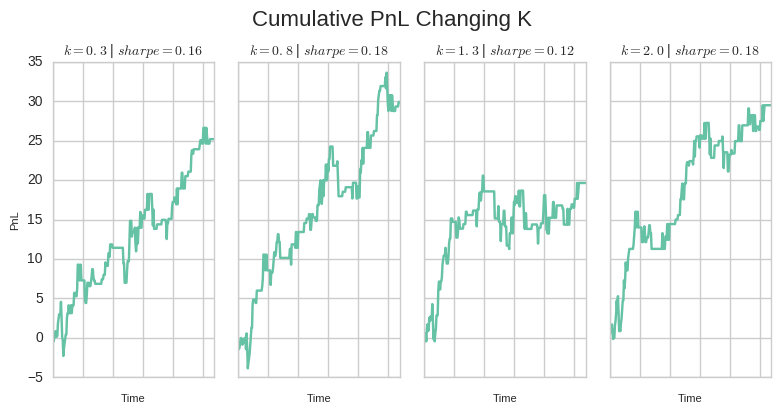
\includegraphics[width=0.75\textwidth]{figures/optimize_k.png}
\caption{\label{fig:optimize_k}The PnL Curves Using Different Value of $k$.}
\end{figure}

When the agent was set to use $k=0.8$ and $k=2.0$, it achieved very similar results and Sharpe ratios. As the variable $k$ control the likelihood of the agent try new actions based on the Q value already observed, I will prefer the smallest value because it improves the chance of the agent to explore. In the figure \ref{fig:optimize_gamma} we  performed the same analysis varying only the $\gamma$:

\begin{figure}[ht]
\centering
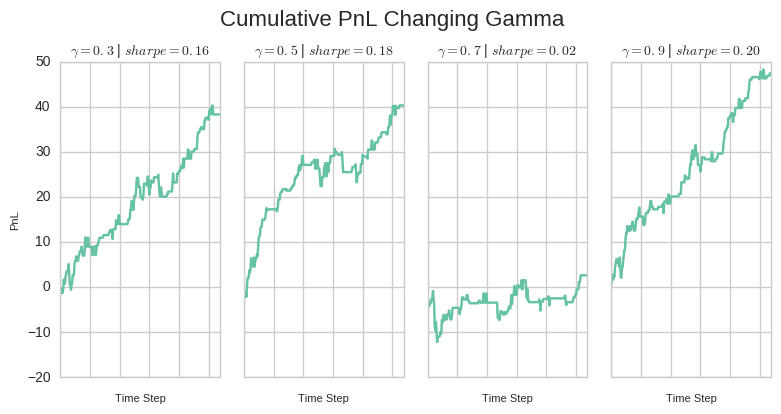
\includegraphics[width=0.75\textwidth]{figures/optimize_gamma.png}
\caption{\label{fig:optimize_gamma}The PnL Curves Using Different Value of $\gamma$.}
\end{figure}

As explained before, as $\gamma$ approaches one, future rewards are given greater emphasis about the immediate reward. When it is zero, only immediate rewards is considered. Despite the fact that the best parameter was $\gamma = 0.9$, I am not comfortable in giving so little attention to immediate rewards. It sounds dangerous when we talk about stock markets. So, I will choose to use $\gamma = 0.5$ arbitrarily in the next tests.

\begin{figure}[ht]
\centering
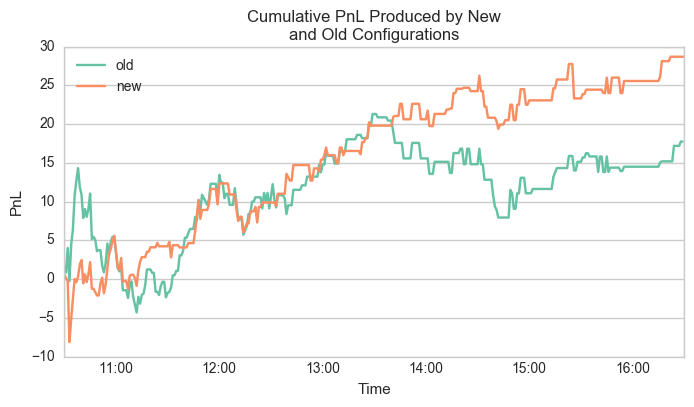
\includegraphics[width=0.75\textwidth]{figures/old_new_comparition.png}
\caption{\label{fig:old_new_comparition}PnL From The First vs. Second Configuration.}
\end{figure}

In the figure \ref{fig:old_new_comparition}, an agent was trained using $\gamma=0.5$ and $k=0.8$ and its performance in out-of-sample test is compared to the previous implementation. In this case, the dataset from 07/16/2016 was used. the current configuration improved the performance of the model. We will discuss the final results in the next section.


%%%%%%%%%%%%%%%%%%%%%%%%%%%%%%%%%%%%%%%%%%%%%%%%%%%%%%%%%%%%%%%%%%%%%%%%%%%%%%%%%%%%%%%%
%% RESULTS
%%%%%%%%%%%%%%%%%%%%%%%%%%%%%%%%%%%%%%%%%%%%%%%%%%%%%%%%%%%%%%%%%%%%%%%%%%%%%%%%%%%%%%%%

\section{Results}
\label{sec:results}

In this section, I will evaluate the final model, test its robustness and compare its performance to the benchmark established earlier.

\subsection{Model Evaluation and Validation}
One of the last questions that remain is if the model can make money in different scenarios. To test the robustness of the final model, I am going to use the same framework in very spaced days.

As each round of training and testing sessions takes 20-30 minutes to complete, I will check its performance just on three different days. I have already used the file of index 15 in the last tests. Now, I am going to use the files with index 5, 25 and 35 to train new models, and use the files with index 6, 26 and 36 to perform out-of-sample tests. In the Figure \ref{fig:pnl_diff_days} we can see how the model performed in different unseen datasets.

\begin{figure}[ht]
\centering
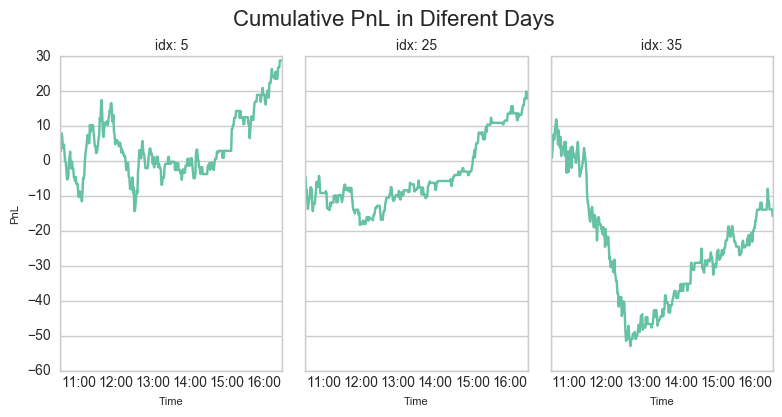
\includegraphics[width=0.75\textwidth]{figures/pnl_diff_days.png}
\caption{\label{fig:pnl_diff_days}PnL When Testing on Different Days.}
\end{figure}

The model was able to make money in two different days after being trained in the previous session to each day. The performance of the third day was pretty bad. However, even wasting a lot of money at the beginning of the day, the agent was able to recover the most of its loss at the end of the session.

Looking at just to this data, the performance of the model looks very unstable and a little disappointing. In the next subsection, we will see why it is not that bad.


\subsection{Justification}
Lastly, I am going to compare the final model with the performance of a random agent. We are going to compare the performance of those agents in the out-of-sample test.

As the learning agent follows strictly the policy learned, I will simulate the operations of this agent on the datasets tested just once. Even though I had run more trials, the return would be the same. However, I will simulate the operations of the random agent $20$ times at each dataset. As this agent can take any action at each run, the performance can be very good or very bad. So, I will compare the performance of the learning agent to the average performance of the random agent.

In the figure \ref{fig:optimal_vs_random_pnl} we can see how much money each one has made in the first dataset used in this project, from 08/16/2016. The learning agent was trained using data from 08/15/2016, the previous day.

\begin{figure}[ht]
\centering
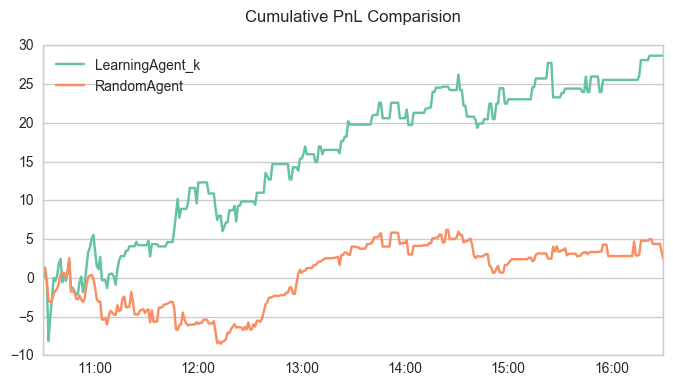
\includegraphics[width=0.75\textwidth]{figures/optimal_vs_random_pnl.png}
\caption{\label{fig:optimal_vs_random_pnl}Performance from Leaning and Random Agent}
\end{figure}

The learning agent greatly outperforms the random agent, the chosen benchmark. Finally, in the figure \ref{fig:pnl_diff_days_compare} I am going to perform the same test using the datasets used in the previous subsection.

\begin{figure}[ht]
\centering
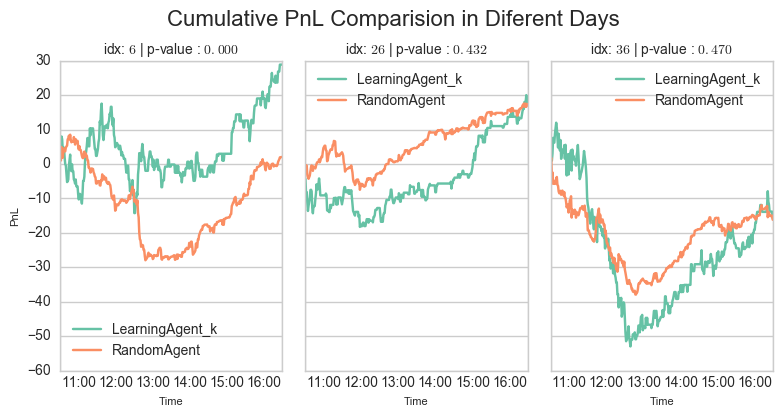
\includegraphics[width=0.75\textwidth]{figures/pnl_diff_days_compare.png}
\caption{\label{fig:pnl_diff_days_compare}Performance from Agents in different Days.}
\end{figure}

In the dataset with index 26 and 36, the random agent outperformed the learning agent most the time, but at the end of these days, the learning agent was able to catch up the random agent performance. In the dataset with index 6, the learning agent outperformed the random agent by a large margin. Curiously, in the worst day of the test, the random agent also performed poorly, suggesting that it wasn't a problem of my agent, but something that has happened on the market.

I believe these results are encouraging because they suggested that using the same learning framework on different days we can successfully find practical solutions that adapt well to new circumstances.

%%%%%%%%%%%%%%%%%%%%%%%%%%%%%%%%%%%%%%%%%%%%%%%%%%%%%%%%%%%%%%%%%%%%%%%%%%%%%%%%%%%%%%%%
%% CONCLUSION
%%%%%%%%%%%%%%%%%%%%%%%%%%%%%%%%%%%%%%%%%%%%%%%%%%%%%%%%%%%%%%%%%%%%%%%%%%%%%%%%%%%%%%%%

\section{Conclusion}
\label{sec:conclusion}

In this section, I will discuss the final result of the model, summarize the entire problem solution and suggest some improvements that could be made.

\subsection{Final Remarks}

In this project, We have proposed the use of the reinforcement learning framework to build an agent that learns how to trade according to the market states and its own conditions. After that the agent's policy was optimized to the previous sessions to the days it would have traded (in the out-of-sample tests), the agent would have been able to generate the result exposed in the figure below.

\begin{figure}[ht]
\centering
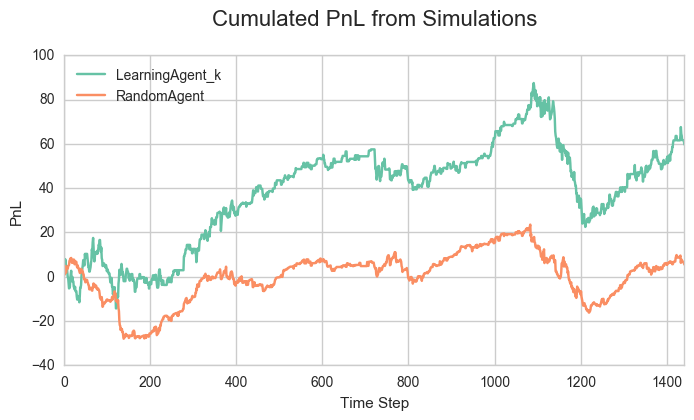
\includegraphics[width=0.75\textwidth]{figures/optm_rand_several_days.png}
\caption{\label{fig:optm_rand_several_days}Performance from Agents in different Days.}
\end{figure}

The chart above shows the accumulated return in four different days generated by the learning agent  and by the random agent. Although the learning agent has not made money all the time, it still beat the performance of the random agent on the period of the tests.

To find the optimal policy we have used Q-Learning, a model-free approach to reinforcement learning. We trained the agent by simulating several runs on the same dataset, allowing the agent to explore the results of different actions on the same environment. So, we have back-tested the policy learned on the same dataset and found out that the policy learned not always converge to a better one. We noticed that this non-convergence could be related to the nature of our problem.

So, we refined the model testing different configurations of the model parameters and compare the PnL of the new policy to the old one back testing them against a different dataset. Finally, after we selected the best parameters, we trained the model in different days and tested against the subsequent sessions.

We compared these results to the returns of a random agent and concluded that our model was significantly better during the period of the tests.

One of the most interesting parts of this project was to define the state representation of the environment. I find out that when we increase the state space too much, it becomes very hard the agent learns an acceptable policy in the number of the trials we have used. The number of trials used was mostly determined by the time it took to run (several minutes)

It was interesting to see that, even clustering the variables using k-means, the agent was still capable of using the resulting clusters to learn something useful from the environment.

Building the environment was the most difficult and challenging part of the entire project. Not just find an adequate structure for build the order book wasn't trivial, but make the environment operates it correctly was difficult. It has to manage different orders from various agents and ensure that each agent can place, cancel or fill orders (or have orders been filled) in the right sequence.

Overall, I believe that the simulation results have shown initial success in bringing reinforcement learning techniques to build algorithmic trading strategies. Develop a strategy that doesn't perform any arbitrage\footnote{Source: \url{https://en.wikipedia.org/wiki/Arbitrage}} and still never lose money is something very unlikely to happen. This agent was able to mimic the performance of an average random agent sometimes and outperforms it other times.


\subsection{Improvement}

bla

%%%%%%%%%%%%%%%%%%%%%%%%%%%%%%%%%%%%%%%%%%%%%%%%%%%%%%%%%%%%%%%%%%%%%%%%%%%%%%%%%%%%%%%%
%% END
%%%%%%%%%%%%%%%%%%%%%%%%%%%%%%%%%%%%%%%%%%%%%%%%%%%%%%%%%%%%%%%%%%%%%%%%%%%%%%%%%%%%%%%%

\bibliographystyle{plain}
% or try abbrvnat or unsrtnat
\bibliography{bibliography/biblio.bib}
\end{document}
